\documentclass[portuguese]{textolivre}

% metadata
\journalname{Texto Livre}
\thevolume{17}
%\thenumber{1} % old template
\theyear{2024}
\receiveddate{\DTMdisplaydate{2024}{8}{8}{-1}}
\accepteddate{\DTMdisplaydate{2024}{10}{27}{-1}}
\publisheddate{\DTMdisplaydate{2024}{11}{5}{-1}}
\corrauthor{Terezinha Marcondes Diniz Biazi}
\articledoi{10.1590/1983-3652.2024.53965}
%\articleid{NNNN} % if the article ID is not the last 5 numbers of its DOI, provide it using \articleid{} commmand 
% list of available sesscions in the journal: articles, dossier, reports, essays, reviews, interviews, editorial
\articlesessionname{articles}
\runningauthor{Biazi}
%\editorname{Leonardo Araújo} % old template
\sectioneditorname{Daniervelin Pereira}
\layouteditorname{João Mesquita}

\title{Estado da arte sobre o uso educacional de dados abertos em artigos internacionais: ensinos superior e básico}
\othertitle{State of the art on the educational use of open data in international articles: higher and basic education}

\author[1,2]{Terezinha Marcondes Diniz Biazi~\orcid{0000-0001-8599-8786}\thanks{Email: \href{mailto:emebiazi@hotmail.com}{emebiazi@hotmail.com}}}
\affil[1]{Universidade Estadual de Campinas, Campinas, SP, Brasil.}
\affil[2]{Universidade Estadual do Centro-Oeste, Guarapuava, PR, Brasil.}

\addbibresource{article.bib}

\begin{document}
\maketitle
\begin{polyabstract}
\begin{abstract}
O objetivo deste estudo foi mapear publicações internacionais sobre o uso educacional de dados abertos nos ensinos superior e básico entre 2013 e 2023. Adotou-se uma abordagem quanti-qualitativa, analisando 58 artigos obtidos de fontes como \textit{Directory of Open Access Journals, Google Scholar, Semantic Scholar, ResearchGate e Connected Papers}. Os critérios de inclusão consideraram o período, o contexto educacional e a língua inglesa. A análise quantitativa focou no volume de publicações, áreas de conhecimento e localização geográfica, enquanto a análise qualitativa investigou desafios e potencialidades da integração de dados abertos na educação. Os resultados revelaram maior concentração de publicações na Europa (43 artigos) e nas áreas de Ciências Exatas e da Terra, especialmente em Ciência da Computação. Observou-se também uma produção acadêmica modesta, com 41 artigos no ensino superior e 17 na educação básica, destacando-se a necessidade de mais estudos sobre o tema. As principais potencialidades incluem o desenvolvimento de competências analíticas e de pensamento crítico, enquanto os desafios envolvem questões de acessibilidade, confiabilidade dos dados e adequação pedagógica. Conclui-se que, embora os dados abertos possuam grande potencial pedagógico, sua aplicação efetiva requer políticas de suporte, capacitação docente e ferramentas adequadas para o contexto educacional, visando uma integração mais ampla e eficaz no currículo escolar.

\keywords{Dados abertos \sep Uso educacional \sep Publicações internacionais \sep Ensino superior \sep Educação básica}
\end{abstract}

\begin{english}
\begin{abstract}
The objective of this study was to map international publications on the educational use of open data in higher and basic education between 2013 and 2023. A quantitative-qualitative approach was adopted, analyzing 58 articles obtained from sources such as the Directory of Open Access Journals, Google Scholar, Semantic Scholar, ResearchGate, and Connected Papers. Inclusion criteria considered the period, educational context, and English language. Quantitative analysis focused on the volume of publications, areas of knowledge, and geographic location, while qualitative analysis explored the challenges and potential of integrating open data into education. The results revealed a higher concentration of publications in Europe (43 articles) and in the fields of Exact and Earth Sciences, particularly in Computer Science. A modest academic production was observed, with 41 articles in higher education and 17 in basic education, highlighting the need for further studies on the subject. The main potential includes the development of analytical and critical thinking skills, while the challenges involve issues of accessibility, data reliability, and pedagogical suitability. It is concluded that, although open data holds great pedagogical potential, its effective application requires support policies, teacher training, and adequate tools for the educational context, aiming for broader and more effective integration into the school curriculum.

\keywords{Open data \sep Educational use \sep International publications \sep Higher education \sep Basic education}
\end{abstract}
\end{english}
\end{polyabstract}

\section{Introdução}
Este artigo tem como objetivo mapear estudos internacionais que investigam o uso de dados abertos como recursos didáticos nos ensinos superior e básico, proporcionando uma visão abrangente do tema. A análise se baseia em pesquisas que exploram dados abertos aplicados a práticas de ensino e aprendizagem \cite{atenas2015,lobo2015,buzato2006,buzato2018,coughlan2019,kukulska-hulme2020}.

Para pesquisadores da área, os dados abertos possuem um potencial significativo como material de apoio em atividades de aprendizagem \cite{coughlan2019}. No entanto, estudos indicam que seu uso ainda é limitado em contextos educativos (Coughlan, 2019; Kukulska-Hulme et al., 2020). Segundo \textcite[p.~387]{coughlan2019}, esses recursos são pouco explorados em currículos escolares, uma vez que 'há uma falta de compreensão generalizada entre educadores sobre o que são dados abertos' e, consequentemente, sobre seu valor pedagógico. De acordo com Atenas et al. (2015), esses dados podem contribuir para o desenvolvimento de habilidades transversais, como letramento digital, pesquisa, pensamento crítico e cidadania global. Há um consenso na academia sobre a necessidade de mais estudos que aprofundem o entendimento das finalidades, contribuições, métodos e técnicas relacionados à pedagogia com dados abertos \cite{bhargava2015,wolff2015,buzato2018,lima-lopes2022,lima-lopes2023}, já que a pesquisa existente ainda é escassa quanto ao uso desses dados em práticas de ensino \cite{coughlan2019}).

Diante do exposto, este artigo busca atender à demanda por mais pesquisas que explorem os dados abertos e suas potencialidades como materiais de ensino e aprendizagem. Considerando a importância de compreender o impacto e as práticas associadas a essa abordagem educacional, propõe-se o seguinte questionamento: 
quais são as tendências e características das publicações internacionais sobre o uso de dados abertos como instrumentos educacionais nos ensinos superior e básico, no período de 2013 a 2023? Para responder a essa questão, definem-se os seguintes objetivos específicos:
\begin{enumerate}
    \item Mapear o panorama quantitativo dos artigos internacionais sobre o uso de dados abertos como recursos educacionais nos ensinos superior e básico.
    \item Identificar as grandes áreas do conhecimento e as áreas básicas de concentração de publicações e autores, bem como as regiões geográficas com maior concentração de produções.
    \item Evidenciar as potencialidades e os principais desafios no uso de dados abertos para fins educacionais, de acordo com a literatura especializada.
\end{enumerate}

A seção a seguir apresenta definições e aplicações dos dados abertos na educação. Em seguida, descrevemos os procedimentos para rastrear, selecionar e documentar os artigos que investigam o uso de dados abertos como instrumentos educacionais nos ensinos superior e básico, no período de 2013 a 2023. A análise dos artigos compilados antecede as considerações finais deste estudo.


\section{Dados abertos na educação: definições e aplicações}\label{sec-normas}
O termo ‘dados’, por sua natureza mutável, é de difícil definição. A organização internacional \textcite{datapop2015}\footnote{Data Pop Alliance é uma aliança internacional que foca em promover o uso ético e eficaz de dados para fomentar o desenvolvimento humano, inclusão social e a tomada de decisões baseadas em evidências.} descreve dados como objetos, variáveis ou informações que podem ser coletados, armazenados e identificados, dependendo do contexto. Para \textcite{silva2007}, dados representam códigos que servem como matéria-prima da informação, ou seja, informações em estado bruto. De acordo com o relatório \cite[p.~24]{world_development_report2021}\footnote{World Development Report (Relatório Mundial de Desenvolvimento) é uma publicação anual do Banco Mundial que analisa temas importantes para o desenvolvimento global, oferecendo dados, análises e recomendações de políticas para promover o crescimento econômico e a redução da pobreza.}, vivemos em uma sociedade orientada por dados, os quais precisam “ser processados, estruturados e analisados para se transformarem em informações” capazes de gerar percepções, escolhas, conhecimentos e soluções, com potencial para melhorar vidas. 

Com os avanços da computação e das tecnologias digitais, fatos, imagens, sons e palavras são convertidos em dados, gerando informações em diferentes contextos e para usos variados. Por exemplo, na área médica, o método de conversão de imagens em dados por meio de técnicas randômicas permite diagnósticos mais precisos após o processamento e a análise dessas informações. Da mesma forma, dados geográficos são empregados para mapear a localização de crimes ou surtos de doenças, utilizando detalhes de referências geoespaciais. Assim, os dados não apenas refletem a complexidade do mundo contemporâneo, mas também se adaptam às transformações tecnológicas e sociais, reforçando seu papel central em diversas áreas do conhecimento e na tomada de decisões \cite{world_development_report2021}.

A conceituação e a utilização de dados abertos em diferentes esferas de atuação são recentes. A \textcite[tradução nossa]{open_knowledge_foundation2005} \footnote{Open Knowledge Foundation: organização internacional que promove o conhecimento aberto em diversas áreas, incluindo dados abertos, governança e educação.} definiu “dados abertos como aqueles que podem ser livremente usados, reutilizados e redistribuídos por qualquer pessoa, desde que sejam atribuídos e compartilhados sob as mesmas condições”. O governo aberto surgiu como uma extensão do Movimento Aberto. Em 2009, países como EUA, Reino Unido, Canadá e Nova Zelândia formalizaram o conceito de dados governamentais abertos ao adotar políticas de transparência e prestações de contas. Atualmente, cerca de 80 países e organizações como as Nações Unidas e o Banco Mundial, compartilham conjuntos de dados abertos de relevância internacional \cite{world_bank_data_catalog2018}\footnote{The World Bank Catalog: plataforma do Banco Mundial que oferece acesso a um vasto conjunto de dados abertos sobre desenvolvimento global.}.

Mas por que precisamos de dados abertos? No contexto de ações governamentais, eles promovem a transparência dos gastos públicos, facilitam o acesso dos cidadãos aos às informações governamentais e permitem o controle das políticas públicas \cite{portal_brasileiro_dados_abertos2012}. Por exemplo, o canadense  David Eaves, especialista em políticas públicas e ativista em dados abertos, destacou que dados abertos ajudaram a expor doações de caridade fraudulentas no valor de US\$ 3,2 bilhões para o governo em 2010 \cite{dataeu2021}\footnote{Data Europe EU: plataforma europeia que disponibiliza dados abertos de diversas áreas, promovendo transparência e acesso à informação na União Europeia.}. Esse fato demonstra como a abertura dos dados pode fortalecer a responsabilidade e a integridade em governos e instituições (\textcite{open_data_charter2015}\footnote{Open Data Charter: iniciativa global que estabelece princípios para a implementação de políticas de dados abertos por governos e organizações.}; \textcite{open_data_institute2017}\footnote{Open Data Institute: organização que promove o uso de dados abertos para estimular a inovação, transparência e desenvolvimento econômico.}). 

Além disso, dados abertos podem resolver problemas e mitigar suas ocorrências, beneficiando a população. Um exemplo é o combate à Covid-19: o projeto \textit{Corona Virus Media Watch}, lançado pela Unesco e pelo Centro de Pesquisa em Inteligência Artificial da Eslovênia, utilizou dados abertos para oferecer uma visão global da pandemia, incluindo casos, reportagens e estatísticas em gráficos para o público \cite{unesco2020}. 

Dados abertos também auxiliam em atividades cotidianas. Ao verificar uma previsão meteorológica \textit{on-line}, usar o GPS (Sistema de Posicionamento Global) para encontrar um endereço ou acessar um aplicativo de transporte, você está utilizando dados abertos \cite{world_bank_data_catalog2018}. 

Como os dados abertos podem ser visualizados? Eles se apresentam de diversas formas, como: mapas (de distribuição de pontos, de calor, de símbolos proporcionais), animações, simulações, gráficos (diagramas, histogramas, cartogramas), nuvens de palavras e grafos \cite{zoss2016,buzato2018}. De modo geral, o uso de dados abertos por governos, sociedade e indivíduos pode auxiliar para aprimoramento da informação em prol da cidadania e do bem comum.

Qual é a relação entre dados abertos e educação? Em consonância com a literatura acadêmica, dados abertos encerram inegável valor educacional pela potencialidade de promover “experiências de aprendizagem autênticas, uma vez que são produzidos a partir de contextos organizacionais concretos \cite[p.~387, tradução nossa]{coughlan2019}. Sob a mesma ótica, \textcite[p.~23, tradução nossa]{atenas2015} afirmam que “educadores que fazem uso de dados abertos no ensino e aprendizagem incentivam os alunos a pensar como pesquisadores, jornalistas, cientistas e como formuladores de políticas e ativistas”. 

Os dados abertos educacionais constituem um campo de estudo recente, com uma literatura em fase inicial de desenvolvimento. De acordo com \textcite{guy2016}, o termo 'dados abertos educacionais' ainda carece de uma definição precisa e pode ser compreendido sob duas vertentes principais: 

\begin{enumerate}
    \item o uso de dados abertos com fins educacionais, ou
    \item a divulgação de dados por instituições de ensino.
\end{enumerate}
 
No primeiro cenário, esses dados podem ser considerados uma subcategoria dos Recursos Educacionais Abertos (REA), nos quais conjuntos de dados são disponibilizados para uso pedagógico. Já no segundo cenário, o foco está na publicação de dados pelas instituições acadêmicas sobre seu próprio desempenho e o de seus alunos, incluindo: dados de referência (como localização das instituições), dados internos (registros de funcionários, orçamento e informações dos alunos), dados curriculares (sobre cursos e objetivos de aprendizagem), dados de interação dos usuários e dados padronizados para comparações, monitoramento de políticas públicas e promoção da transparência \cite{penteado2017,penteado2019,alcantara2020}.  Este artigo concentra-se na primeira vertente, explorando como os dados abertos podem ser aplicados no contexto educacional como recursos pedagógicos, enriquecendo o processo de ensino e aprendizagem.

No cenário pedagógico, os dados abertos têm sido associados aos REA, possibilitando que professores e alunos acessem e manipulem informações do mundo real em atividades de ensino e aprendizagem. O uso desses conjuntos de dados como REA permite que os alunos aprendam e experimentem a partir dos mesmos materiais brutos utilizados por pesquisadores, governos, sociedade civil, organizações internacionais e formuladores de políticas. Sua aplicação na educação é destacada pelo sexto princípio da Carta de Dados Abertos, que incentiva o uso dessas informações para o desenvolvimento inclusivo e a inovação. O princípio enfatiza a importância de “engajar escolas e instituições de ensino superior para aumentar a pesquisa com dados abertos e integrar o letramento em dados nos currículos educacionais” \cite{open_data_charter2015} (\textit{principle 6}). Embora não seja evidente o grau de prioridade dado a esse aspecto por países e cidades que adotaram a Carta, já existem iniciativas que estabelecem essa prática como REA em diversos projetos. Eles podem desempenhar um papel fundamental em atividades de aprendizado baseadas em pesquisa e em cenários práticos, contribuindo para o desenvolvimento de competências informacionais, estatísticas, científicas, midiáticas, políticas e de pensamento crítico dos alunos \cite{wolff2015,atenas2019}.

Os estudos de \textcite{atenas2015,lima-lopes2022} destacam essa conexão, mostrando como a integração de dados abertos e da ciência aberta como REA pode promover práticas pedagógicas mais inclusivas, colaborativas e alinhadas às necessidades do contexto educacional.

\textcite{atenas2015} argumentam que, embora os debates sobre dados abertos e educação aberta tenham avançado de forma separada, os dados abertos podem ser considerados uma forma de REA. Conforme definido pela \textcite[p.~1]{unesco2012}, REA incluem "materiais de ensino, aprendizagem e investigação em quaisquer suportes, em domínio público ou publicados sob licença aberta, permitindo acesso, uso, adaptação e redistribuição”. Mesmo não criados originalmente para fins educacionais, esses dados têm potencial para serem utilizados como REA e, portanto, devem ser integrados à educação. \textcite{atenas2015} defendem que, além do acesso a dados globais, é essencial proporcionar acesso a dados acadêmicos utilizando metodologias de pesquisa aplicadas em sala de aula, o que requer políticas que incentivem sua disponibilização institucional e promovam abordagens de pesquisa multidisciplinares. Integrar dados abertos nos currículos do ensino superior pode desenvolver o pensamento crítico, o rigor acadêmico e a alfabetização em dados, além de melhorar a empregabilidade dos alunos. Esses dados também oferecem oportunidades para o engajamento cívico dos estudantes, por meio de atividades projetadas para desenvolver habilidades de cidadania. Para promover o uso eficaz de dados abertos na educação, é essencial definir resultados de aprendizagem, preparar portais de dados acessíveis e capacitar os alunos no uso de softwares de análise. Os autores apresentam exemplos de diferentes níveis de especialização em atividades de pesquisa com dados abertos e sugerem diretrizes para promover o engajamento cívico em diversos níveis de competência. No entanto, ainda há lacunas na integração entre dados abertos, REA e o desenvolvimento de competências, o que ressalta a necessidade de uma maior conexão entre as práticas de dados abertos e a educação.

\textcite{lima-lopes2022} destaca a importância de integrar a Ciência Aberta (CA) à Educação, propondo que seus resultados sejam tratados como Recursos Educacionais Abertos. O autor argumenta que práticas como publicação aberta, dados abertos e código aberto podem transformar o ensino e a aprendizagem, especialmente na Linguística Aplicada, favorecendo práticas pedagógicas mais inclusivas, baseadas na pesquisa e no conhecimento local. O autor explora as implicações da CA para a Linguística Aplicada, sugerindo que essas práticas aumentam a replicabilidade e a colaboração na área, ao mesmo tempo em que desafiam o modelo científico tradicional, centrado na competição individual e na propriedade intelectual. Ele propõe que a integração da CA à educação linguística deve focar em três aspectos principais: valorização do conhecimento linguístico local, inclusão da pesquisa na formação de professores e desenvolvimento de uma formação tecno-filosófica crítica. O estudo conclui que a CA tem o potencial de democratizar o acesso ao conhecimento e integrar a sociedade à produção científica, promovendo uma educação mais aberta, crítica e alinhada às necessidades sociais.

Em 2015, o grupo \textit{Open Education Working Group} (Grupo de Trabalho em Educação Aberta)\footnote{Open Education Working Group: iniciativa da Open Knowledge Foundation que promove o uso de dados e recursos educacionais abertos para melhorar o ensino e a aprendizagem.} lançou o livro \textit{Open data as open educational resources: case studies of emerging practice} \cite{atenas2015}. Nele, diversos autores propõem atividades que podem ser implementadas por educadores em escolas e universidades para incentivar o uso de dados abertos em iniciativas de pesquisa. A obra reúne exemplos e práticas recomendadas sobre como utilizar dados reais de estudos e de projetos nacionais e internacionais, promovendo o letramento em dados e o pensamento crítico através da colaboração entre alunos, pesquisadores e acadêmicos. Um dos casos destacados no livro é o uso de dados abertos como REA pela \textit{Open Data School} (Escola de Dados Abertos)\footnote{Open Data School, na Rússia: escola que promove o uso de dados abertos por meio de cursos, \textit{workshops} e seminários voltados para educação e cidadania.} na Rússia, que promove palestras e seminários conduzidos por especialistas relacionados a essa temática. Outros exemplos práticos incluem o projeto \textit{Open Linked Data} (Dados Abertos Massivos)\footnote{Projeto Open Linked Data, da Universidade Técnica Particular de Loja: iniciativa que compartilha resultados de pesquisa sobre tecnologia de dados conectados, promovendo acesso aberto e uso educacional.} da Universidad Técnica Particular de Loja, no Equador, que compartilha resultados de pesquisa sobre tecnologia de Dados Conectados para estudantes, pesquisadores e educadores; e o \textit{Monithon}\footnote{Monithon é uma combinação das palavras "monitor" e "marathon" e se refere a uma iniciativa italiana que combina a monitoria cidadã de projetos públicos com atividades de investigação participativa. O objetivo do Monithon é engajar cidadãos, estudantes e pesquisadores na coleta e análise de dados abertos para monitorar a execução de projetos de desenvolvimento e políticas públicas, promovendo a transparência e a responsabilidade governamental. Ele faz parte de um esforço mais amplo de cidadania ativa e uso de dados abertos para o bem comum.}, na Itália, que exemplifica o aprendizado prático, no qual cidadãos e estudantes universitários, junto com pesquisadores e formuladores de políticas, monitoram projetos de desenvolvimento por meio da análise de dados abertos \cite{atenas2019}.

A promoção do uso de dados abertos como REA está diretamente relacionada ao desenvolvimento do letramento em dados. Recentemente, a Iniciativa Latino-Americana de Dados Abertos criou um programa de capacitação voltado para acadêmicos, visando o uso de dados abertos no ensino e aprendizado. Esse programa tem como objetivo ajudar os participantes a adquirir as competências necessárias para atuar em uma sociedade cada vez mais orientada por dados, incluindo a construção de conhecimento e a análise crítica de informações de diversas fontes \cite{atenas2019}.

O letramento em dados emerge como um conceito central nas discussões sobre educação, sendo abordado de forma distinta por \textcite{bhargava2015,lima-lopes2023}, que tratam do desenvolvimento de competências analíticas e críticas, enquanto \textcite{coughlan2019} foca especificamente no uso de dados abertos como recursos educacionais, enfatizando sua integração no ensino.

\textcite{bhargava2015} argumentam que o ensino baseado em dados não apenas melhora a compreensão analítica dos alunos, mas também os prepara para enfrentar desafios sociais e econômicos reais. Eles definem a alfabetização em dados como a capacidade de compreender, manipular, analisar e argumentar com dados, abrangendo tanto a interpretação do que os dados representam quanto sua aplicação para sustentar narrativas mais amplas. Os autores propõem princípios pedagógicos para o desenvolvimento de ferramentas e atividades voltadas para essa competência. Eles destacam que, embora o trabalho com dados seja essencial no século 21, muitas ferramentas existentes priorizam a eficiência prática em detrimento de um aprendizado significativo. Para promover um aprendizado efetivo, os autores defendem a criação de ferramentas que sejam focadas, guiadas e expansíveis, ou seja, projetadas para facilitar o aprendizado progressivo e estimular a exploração crítica dos dados pelos alunos. 

O texto de \textcite{lima-lopes2023} aborda as contribuições do letramento de dados para o letramento científico no campo das ciências da linguagem, com ênfase na Linguística Aplicada. O autor explora como o crescente papel dos dados na sociedade pode influenciar o ensino e a pesquisa em linguística. Ele destaca a importância de entender criticamente os processos de extrativismo de dados e o capitalismo de vigilância, apresentando o letramento de dados como uma ferramenta de resistência e transformação epistemológica. O artigo propõe um modelo de Letramento de Dados que inclui habilidades como aquisição, análise, representação e interpretação de dados, enfatizando o uso crítico de tecnologias e mídias. A abordagem sugere que a análise de dados pode contribuir para uma educação científica mais democrática e adaptada às necessidades locais. O texto também discute como os dados podem ser utilizados para criar novas narrativas, desafiando as perspectivas dominantes e ampliando o entendimento da linguagem em seus contextos sociais.

\textcite{coughlan2019} explora o potencial dos dados abertos como recursos em atividades de aprendizado. A pesquisa investiga o uso inicial de dados abertos na educação, entrevistando educadores que adotaram essa abordagem em diferentes projetos e contextos de ensino. Foram analisados os motivos para o uso de dados abertos, o design adequado das atividades e os desafios práticos enfrentados pelos professores. Os resultados destacam a falta de conscientização e de uso coordenado dos dados abertos entre os educadores, muitos dos quais os confundem com dados gratuitos sem licença aberta. Os casos de ensino analisados sugerem uma tendência para métodos de aprendizado baseados em projetos, que utilizam dados abertos para desenvolver habilidades de análise, pensamento crítico e alfabetização em dados. O artigo também propõe um quadro conceitual para apoiar uma integração mais ampla de dados abertos na educação, conectando-os a conceitos pedagógicos existentes, como aprendizado baseado em investigação, personalização e autenticidade. 

\textcite{coughlan2019} ressalta que os dados abertos podem ser um recurso autêntico e relevante para atividades educativas, promovendo o engajamento público e o aprendizado em diversas disciplinas, ao mesmo tempo em que aproveitam os interesses pessoais dos alunos para fomentar a alfabetização em dados. No entanto, o uso limitado de dados abertos na educação é atribuído a desafios como a falta de competências e recursos adequados. Embora novas ferramentas estejam emergindo para simplificar o uso de dados abertos, ainda persistem barreiras de acessibilidade. Para superá-las, o estudo sugere soluções colaborativas e um quadro conceitual que facilita a integração dos dados abertos no ensino. A participação ativa das organizações que compartilham dados e a criação de parcerias entre educadores, alunos e produtores de dados podem tornar o aprendizado mais autêntico. Além disso, é essencial que educadores e tecnólogos adaptem os dados ao contexto educacional. Para aumentar a eficácia dos dados abertos no aprendizado, é necessário projetar atividades que aproveitem suas qualidades e alinhem-se às pesquisas e práticas pedagógicas existentes, com o quadro conceitual proposto servindo como ponto de partida para direcionar esses esforços.

Para concluir, é evidente que o uso de dados abertos na educação possui um potencial transformador, tanto em termos de práticas pedagógicas quanto de letramento de dados. Seja integrando-os como REA, promovendo o pensamento crítico e o engajamento cívico, ou desenvolvendo uma compreensão mais ampla das questões sociais e científicas, a adoção de dados abertos pode enriquecer significativamente o ensino e a aprendizagem. No entanto, para que esse potencial seja plenamente alcançado, é crucial investir em políticas de suporte, na capacitação de educadores e em ferramentas acessíveis que adaptem esses dados ao contexto educacional. A pesquisa deve continuar a explorar maneiras de superar os desafios existentes, facilitando a conexão entre as comunidades de educação aberta e dados abertos, de modo a garantir uma integração mais ampla e eficaz desses recursos no currículo educacional \cite{atenas2015,bhargava2015,atenas2019,coughlan2019,lima-lopes2022,lima-lopes2023}.


\section{Caminhos metodológicos da pesquisa}\label{sec-conduta}
A presente pesquisa adotou uma abordagem exploratória, descritiva e de natureza quanti-qualitativa, cada uma escolhida com um propósito específico. O foco está em explorar as características e tendências das publicações sobre o uso de dados abertos na educação, o que justifica o caráter exploratório do estudo. É descritiva uma vez que buscou apresentar um panorama detalhado dos dados coletados e das informações disponíveis. 
A combinação de métodos permitiu uma análise mais abrangente: o aspecto quantitativo foi utilizado para mapear e mensurar o volume de publicações, áreas de conhecimento e localização geográfica, enquanto o qualitativo analisou as potencialidades, desafios e práticas associadas ao uso de dados abertos no ensino, aprofundando a compreensão das narrativas e interpretações presentes nos artigos selecionados.

O \textit{corpus} foi constituído por um levantamento e análise de artigos internacionais publicados entre 2013 e 2023, abordando a interseção da Educação e Tecnologia, especificamente sobre o uso educacional de dados abertos (ver \Cref{fig1}). O processo metodológico foi delineado por meio da coleta, tratamento e análise provenientes das seguintes fontes: \textit{Directory of open Access Journals, Google Scholar, Semantic Scholar, Research Gate e Connected Papers}. Foram adotados os seguintes critérios de inclusão: 1) delimitação temporal entre 2013 e 2023; 2) produções em áreas/linhas de pesquisa alinhadas à natureza interdisciplinar de Educação e Tecnologias; 3) pesquisas em língua inglesa e 4) aplicação de chaves de busca avançada: ‘\textit{educational use of open data}’ OU ‘\textit{open data for teaching and learning}’ OU ‘\textit{open data for higher education}’ OU ‘\textit{open data for primary education}’ OU ‘\textit{open data for secondary school}’. 

A coleta resultou em 65 artigos, submetidos a uma leitura integral para categorização adequada, já que os resumos se mostraram insuficientes. Durante a filtragem, sete artigos foram excluídos devido ao distanciamento do escopo pretendido ou à inacessibilidade do conteúdo completo. O \textit{corpus} final compreendeu 58 artigos, documentados em duas planilhas - uma para artigos de ensino superior e outra para artigos de nível básico -, abrangendo 11 critérios: ano de publicação, autor, título, universidade, área de concentração, linha de pesquisa, palavras-chave, objetivo, temática, contexto de investigação e principais resultados. As planilhas com os dados das pesquisas estão disponibilizadas online para consulta e uso abertamente em: \url{https://zenodo.org/badge/DOI/10.5281/zenodo.14031155.svg}.

\begin{figure}[h]
\centering
\begin{minipage}{0.75\linewidth}
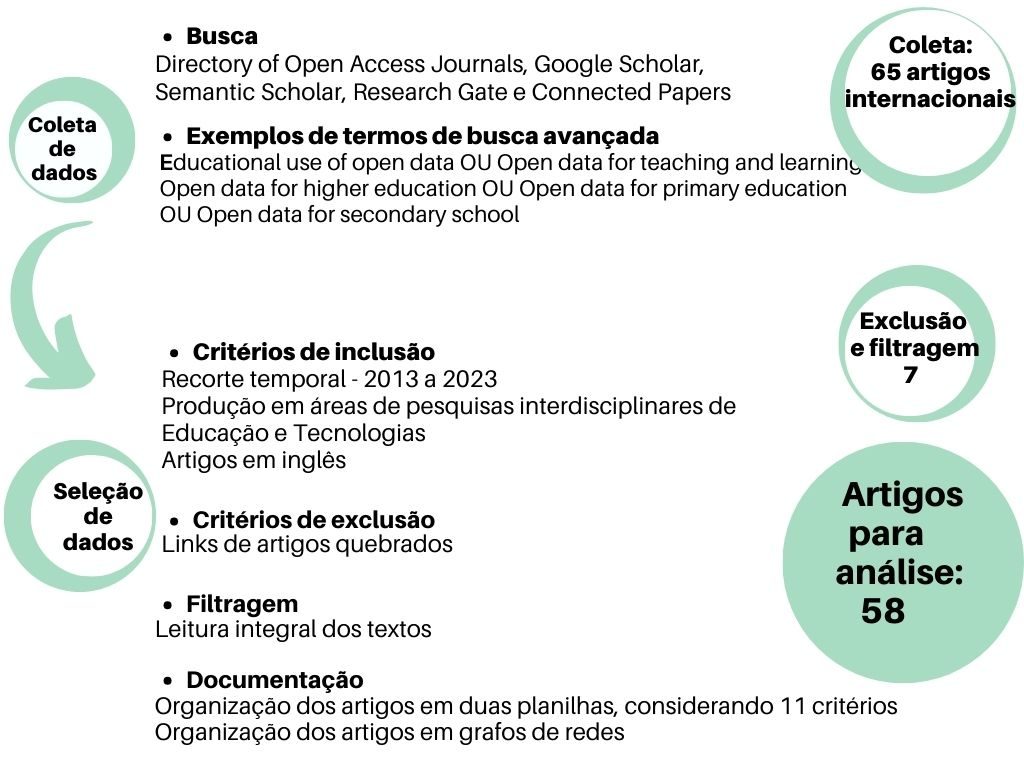
\includegraphics[width=\linewidth]{Fig1.png}
\caption{Etapas de coleta e seleção dos dados.}
\label{fig1}
\source{Elaborado pela autora.}
\end{minipage}
\end{figure}

Os artigos analisados foram organizados em grafos de redes para facilitar a visualização e a interpretação dos resultados (ver \Cref{fig2}). Cada nó na rede corresponde a um artigo específico, enquanto as linhas que conectam os nós indicam relações diversas, como citações, influências teóricas e temas compartilhados. Essa configuração permitiu não apenas um agrupamento temático mais preciso das referências, mas também um mapeamento visual mais claro do \textit{corpus} de análise.

\begin{figure}[h]
\centering
\begin{minipage}{0.75\linewidth}
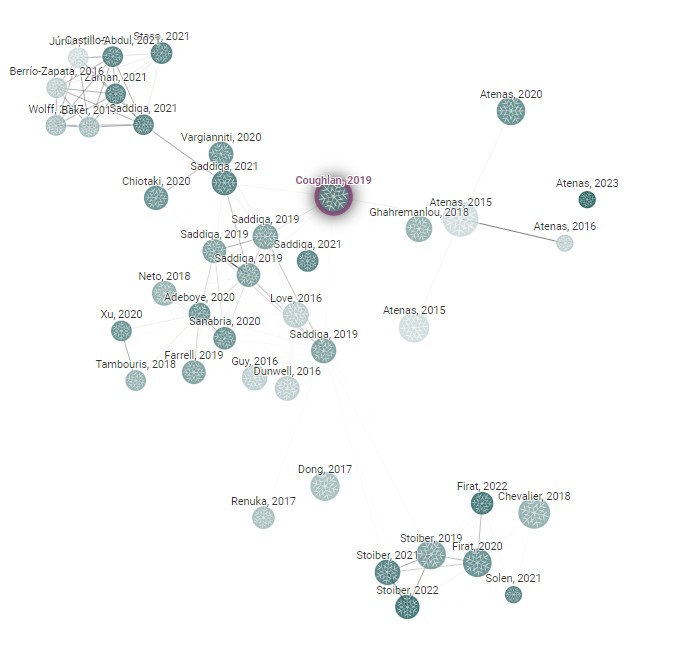
\includegraphics[width=\linewidth]{Fig2.png}
\caption{Representação visual do \textit{corpus} de análise.}
\label{fig2}
\source{Elaborado pela autora.}
\end{minipage}
\end{figure}

A delimitação temporal de 2013 a 2023 foi estabelecida para a busca de artigos na educação superior e básica.
No entanto, é importante ressaltar uma disparidade nesse recorte temporal entre as duas esferas. Enquanto os artigos sobre educação superior cobrem integralmente o período de 2013 a 2023, os relacionados à educação básica têm início apenas em 2015, estendendo-se até 2023. Essa discrepância temporal entre as duas áreas de ensino é um fator relevante a ser considerado na análise comparativa dos dados.

Conforme mencionado, esta pesquisa adotou tanto o viés quantitativo quanto o qualitativo no tratamento dos dados. A análise quantitativa envolveu três etapas: 1) quantificação do volume de produções entre 2013 e 2020 nos ensinos superior e básico; 2) distribuição das produções por áreas de conhecimento dos autores; e 3) estimativa das produções por continente. A análise qualitativa, por sua vez, focou na identificação dos desafios e potencialidades do uso de dados abertos como recursos educacionais.

A análise dos artigos foi conduzida com base na metodologia de análise de conteúdo proposta por \textcite{krippendorff1980}, escolhida por sua capacidade de explorar não apenas o volume de publicações, mas também os temas e significados associados à integração de dados abertos na educação. Essa abordagem permitiu identificar como os dados abertos são aplicados nos estudos analisados, revelando potenciais, desafios e interpretações que transcendem a simples contagem de artigos. Com isso, a análise de conteúdo contribuiu para uma compreensão mais crítica e aprofundada das práticas de uso de dados abertos no campo educacional.

\section{Respondendo aos objetivos de pesquisa}\label{sec-fmt-manuscrito}
Nesta seção, são abordados sistematicamente os três objetivos estabelecidos para esta pesquisa. Cada objetivo é tratado de forma individual, com uma análise detalhada dos dados coletados, visando proporcionar uma compreensão ampla e aprofundada do panorama estudado.

\subsection{Objetivo 1 – apresentar o panorama quantitativo dos artigos internacionais sobre o uso de dados abertos como recursos educacionais nos ensinos superior e básico}\label{sec-formato}
Ocorreu uma flutuação no volume de publicações de artigos internacionais sobre o uso de dados abertos no ensino superior entre 2013 e 2023, totalizando 41 publicações (ver \Cref{fig3}). Durante esse período, registraram-se anos com uma incidência mais expressiva de publicações, contrastando com períodos em que o número de artigos foi menos proeminente. 

Em 2013, foi publicado um artigo, seguido por um aumento para dois artigos em 2014. O ano de 2015 marcou uma ascensão significativa, com 10 publicações, contudo, em 2016, esse número caiu para oito. Em 2017, a quantidade de artigos foi reduzida pela metade, com quatro publicações. Já em 2018, observou-se um ressurgimento, totalizando seis artigos. No ano subsequente, houve uma queda para quatro artigos. Os anos 2020 e 2021 apresentaram uma equiparação, com um artigo cada. Por fim, 2022 e 2023 mantiveram-se estáveis, com dois artigos publicados em cada ano. Essa análise temporal evidencia a variabilidade na produção acadêmica ao longo do período em questão.  

\begin{figure}[h!]
\centering
\begin{minipage}{0.75\linewidth}
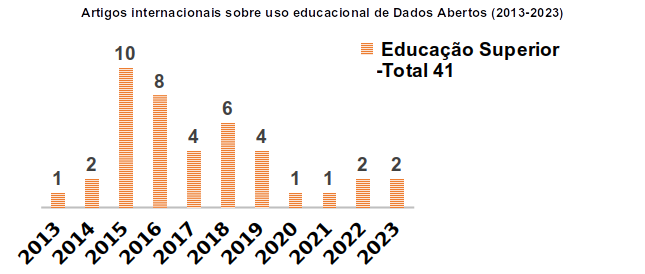
\includegraphics[width=\linewidth]{Fig3.png}
\caption{Produções de artigos por ano de publicação.}
\label{fig3}
\source{Elaborado pela autora.}
\end{minipage}
\end{figure}

Reitera-se que, diferentemente do ensino superior, as publicações de artigos relacionados à educação básica iniciaram apenas em 2015, estendendo-se até 2023 (ver \Cref{fig4}). Nota-se uma variação significativa, com alguns anos apresentando um volume expressivo de publicações, enquanto em outros a disseminação de artigos foi mínima, para não dizer quase inexistente. 

No total, foram publicados 17 artigos sobre educação básica entre 2015 e 2023. Em 2015, registrou-se apenas um artigo, enquanto 2016 apresentou um aumento para dois artigos. Em 2018, o número de publicações voltou ao mesmo patamar de 2015, com um único artigo. O ano mais produtivo foi 2019, com cinco publicações. Em 2020, houve uma redução para dois artigos, seguida de uma recuperação em 2021, que contou com quatro publicações. Nos anos de 2022 e 2023, o volume manteve-se estável, com um artigo publicado em cada ano. Essa análise temporal evidencia a oscilação na produção acadêmica ao longo do período investigado no âmbito da educação básica.

\begin{figure}[h]
\centering
\begin{minipage}{0.75\linewidth}
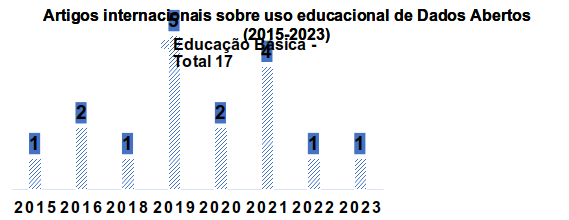
\includegraphics[width=\linewidth]{Fig4.png}
\caption{Produções de artigos por ano de publicação.}
\label{fig4}
\source{Elaborado pela autora.}
\end{minipage}
\end{figure}

\subsection{Objetivo 2 - identificar as grandes áreas do conhecimento e as áreas básicas de concentração de publicações e autores, bem como as regiões geográficas com maior concentração de produções}\label{sec-modelo}
Apresentamos de maneira decrescente o quantitativo de autores distribuídos em suas respectivas áreas de especialização (ver \Cref{fig5}). Vale destacar que a composição dos artigos variou em termos de autoria, oscilando entre dois e quatro autores por publicação.

No âmbito das Ciências Exatas e da Terra, identificamos um total de 52 autores, distribuídos nas seguintes subáreas: quarenta na Ciência da Computação, dez na Estatística e dois em Geociências. Seguindo no sentido horário da figura, as Ciências Humanas somam 22 autores, com destaque para a equivalência quantitativa de dez autores nas disciplinas de Educação e Arqueologia, respectivamente, enquanto as áreas de Geografia e Sociologia contam com dois autores cada. 

A categoria das Ciências Sociais Aplicadas abrange 13 autores, sendo seis na Comunicação, cinco na Ciência da Informação e um autor nas áreas de Direito e Administração Pública. No campo das Engenharias, registram-se três autores: dois na Engenharia Industrial e um na Engenharia Médica. Por fim, a área de Linguística, Letras e Artes é representada por um autor. Observa-se, assim, que a área de conhecimento mais predominante em termos de publicações durante o período analisado é Ciências Exatas e da Terra, com uma ênfase especial em autores especializados em Ciência da Computação.

\begin{figure}[h]
\centering
\begin{minipage}{0.75\linewidth}    
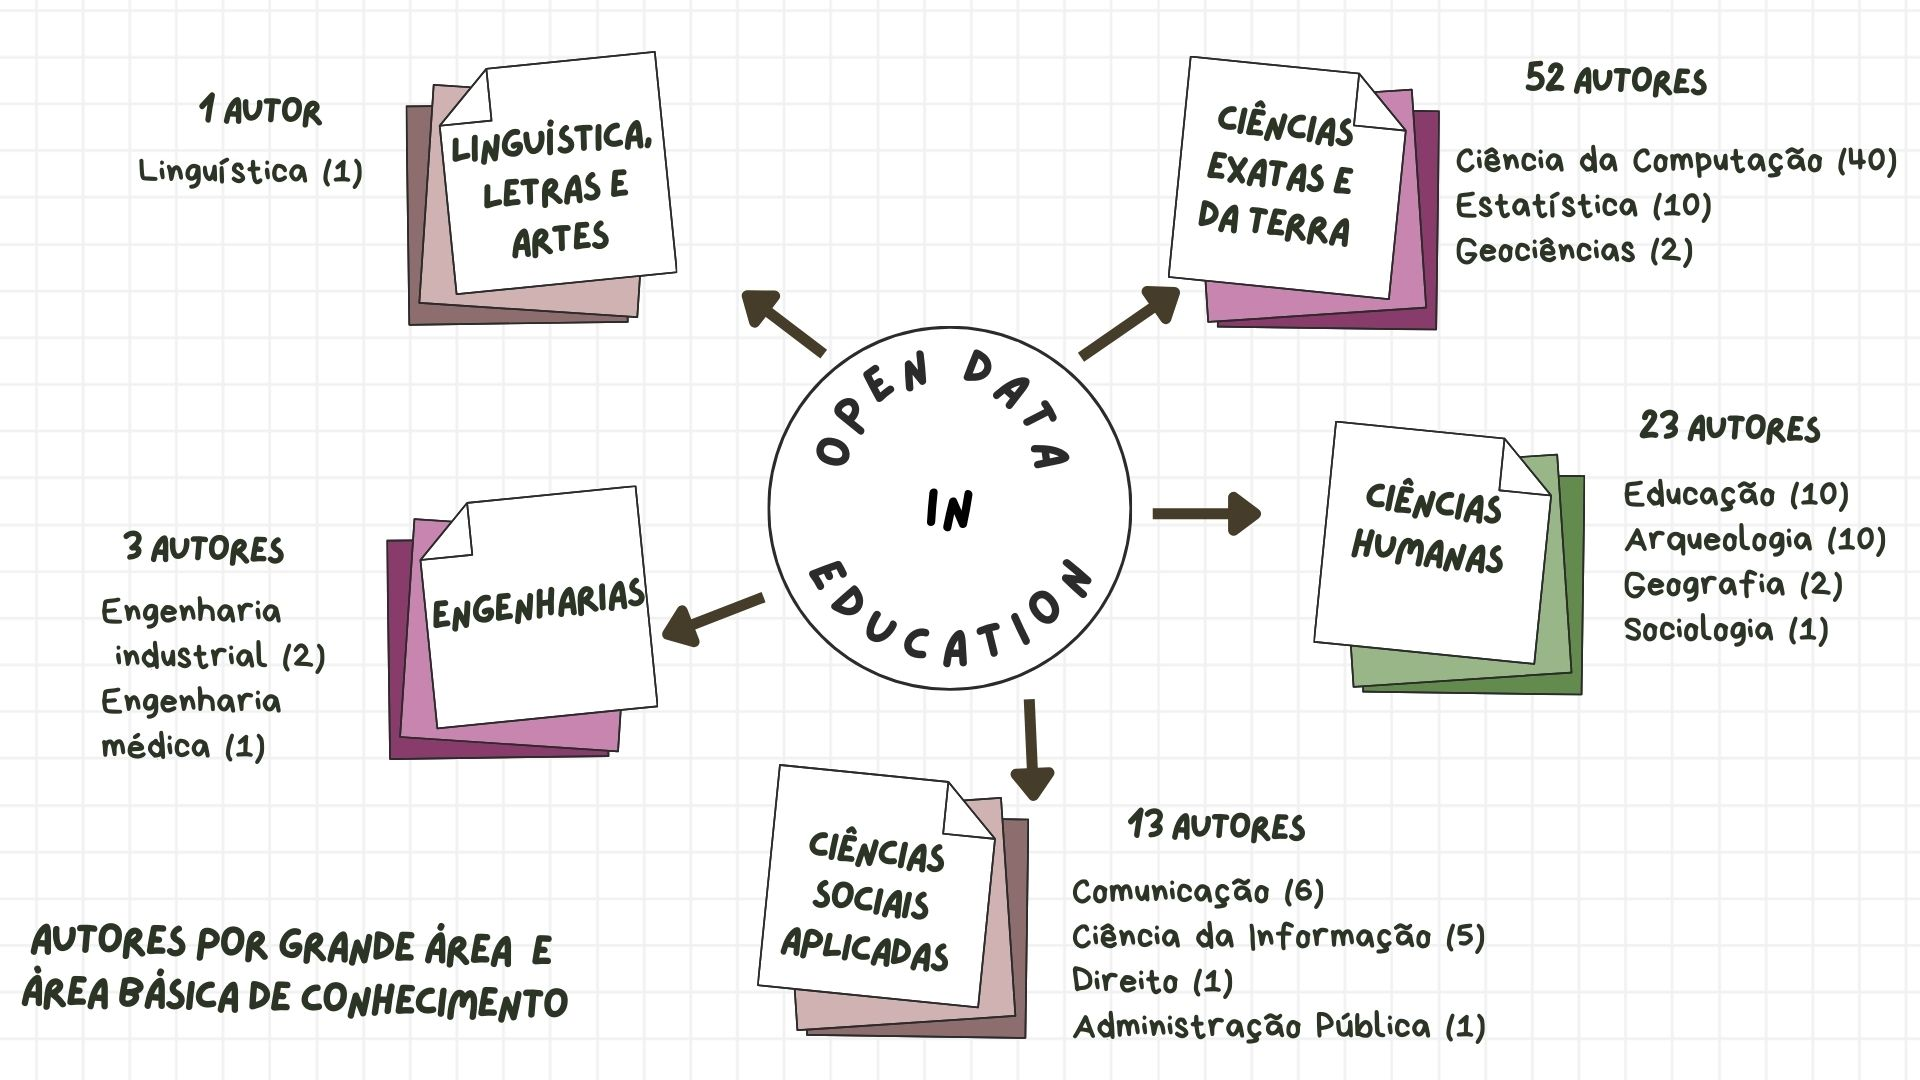
\includegraphics[width=\linewidth]{Fig5.png}
\caption{Autores por grande área e área básica de conhecimento.}
\label{fig5}
\source{Elaborado pela autora.}
\end{minipage}
\end{figure}

As publicações sobre o uso educacional de dados abertos entre 2013 e 2023 abrangem cinco continentes, tanto na educação superior quanto na básica (ver \Cref{fig6}). Destaca-se a predominância da Europa, que acumula 43 artigos publicados, contrastando com os outros continentes, que apresentam números consideravelmente menores. As Américas contabilizam 7 artigos, a Ásia registra 4, enquanto a África conta com 3 publicações. A Oceania, por sua vez, é representada por apenas 1 artigo. Assim, percebe-se que o continente europeu se destaca de maneira significativa no panorama mundial, evidenciando sua liderança na produção acadêmica sobre o tema.

\begin{figure}[h]
\centering
\begin{minipage}{0.75\linewidth}
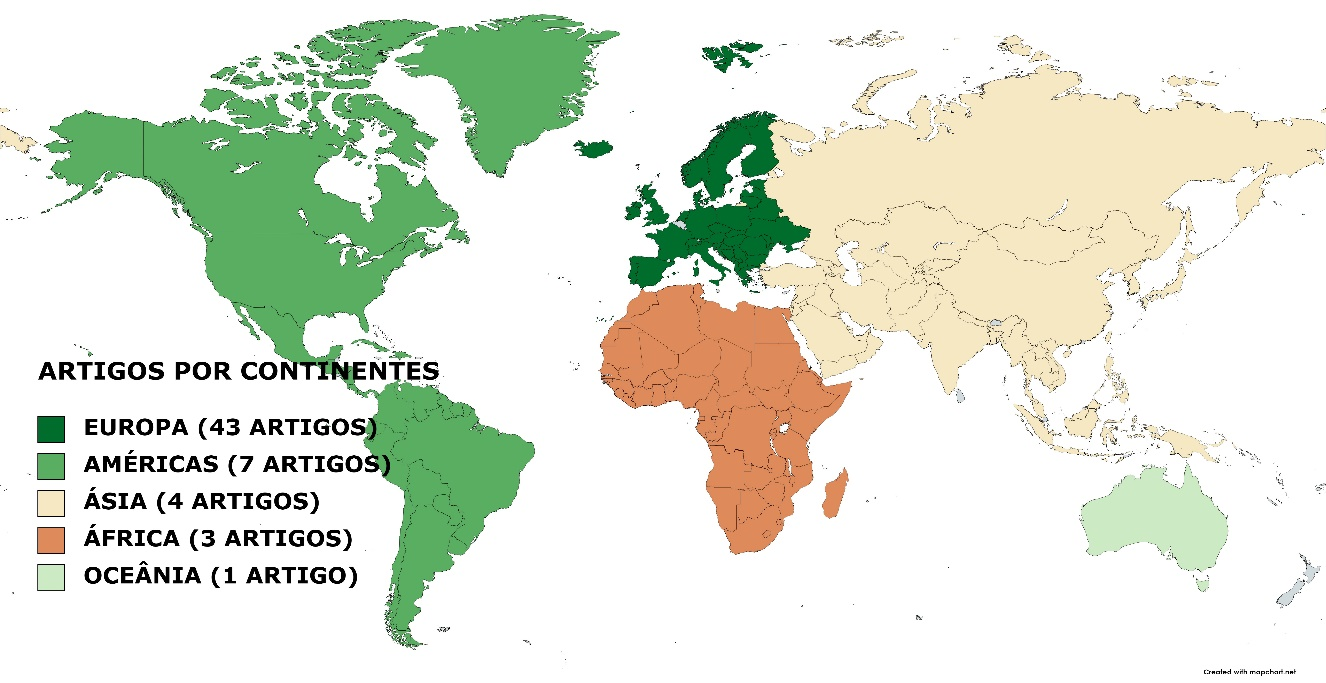
\includegraphics[width=\linewidth]{Fig6.png}
\caption{Publicação de artigos por continente.}
\label{fig6}
\source{Elaborado pela autora.}
\end{minipage}
\end{figure}

\subsection{Objetivo 3 – evidenciar as potencialidades e os principais desafios no uso de dados abertos para fins educacionais, de acordo com a literatura especializada.}  
Listamos a seguir algumas capacidades dos dados abertos que podem ser otimizadas como recursos pedagógicos, contribuindo para o processo de ensino e aprendizagem:

\textbf{Aprendizagem Contextualizada com Dados Reais} - a perspectiva de trabalho didático com dados abertos fornece aos alunos a experiência de trabalhar com as mesmas matérias-primas de cenários do mundo real que cientistas e formuladores de políticas utilizam \cite{atenas2015,kukulska-hulme2020}, articulando a aprendizagem com questões do mundo real \cite{kasl1997,barron1998,hmelo2004,davies2010}. Conforme pontuado por \textcite{atenas2015}, dados abertos podem desempenhar um papel essencial em práticas educacionais centradas em pesquisa e situações contextualizadas, contribuindo para o avanço das competências dos alunos nas esferas informativa, estatística, científica, midiática, política e de pensamento crítico. Ao envolver-se com conjuntos de dados do mundo real, os estudantes têm a oportunidade de aprimorar suas capacidades de narrativa e pesquisa, aplicando habilidades analíticas, colaborativas e cívicas na utilização de informações para abordar desafios concretos.

\textbf{Desenvolvimento progressivo de competências em visualização e análise de dados} - a incorporação de práticas educacionais com dados abertos amplia formas de aquisição de informações contextualizadas, possibilitando aos alunos o envolvimento com problemas contemporâneos e com necessidades locais e globais da sociedade \cite{atenas2015,coughlan2019}. No âmbito da manipulação de visualização de dados, as diretrizes propostas por \textcite{atenas2015} abrangem quatro estágios progressivos. No estágio inicial, os estudantes têm a capacidade de criar gráficos e tabelas. Ao atingir o estágio intermediário, os alunos podem empregar ferramentas online para a elaboração de infográficos simples. Avançando para o estágio proficiente, os estudantes podem utilizar softwares de design gráfico na criação de infográficos mais elaborados, e, finalmente, no estágio avançado, os alunos têm a habilidade de empregar técnicas avançadas de visualização de dados para apresentar suas descobertas por meio de modelagem estatística complexa.

\textbf{Motivação e aprendizagem global com dados contextualizados} - o trabalho com dados reais e contextualizados pode ter um “forte impacto motivacional para alunos que desejam entender o que está acontecendo em sua comunidade local ou em partes distintas do globo” \cite[p.~19, tradução nossa]{kukulska-hulme2020}. Estudantes globalmente têm a oportunidade de integrar seu conhecimento local, participando de uma experiência de aprendizado conjunta. Um exemplo de atividade é a análise de dados relacionados às estatísticas educacionais ou de saúde de seus países, possibilitando comparações com outros locais. Essa abordagem revela-se especialmente apropriada para a aprendizagem em larga escala por meio de Cursos \textit{Online} Abertos e Massivos (Moocs) ou ao engajamento em iniciativas de pesquisa cidadã que promovem a participação generalizada na ciência. Essas práticas capacitam os cidadãos, auxiliando-os no desenvolvimento das habilidades de raciocínio e resolução de problemas comumente utilizadas por cientistas \cite{kukulska-hulme2020}.

Listamos, a seguir, os principais desafios enfrentados no contexto do uso educacional de dados abertos, conforme evidenciado pela literatura internacional. \textcite{kukulska-hulme2020} apontam que a integração de dados abertos na educação enfrenta obstáculos semelhantes aos encontrados na aplicação de \textit{big data} na pesquisa educacional, como detalhado no relatório ‘Pedagogia Inovadora de 2017’\footnote{Pedagogia Inovadora de 2017: Relatório da Open University que explora tendências emergentes e práticas inovadoras em educação, incluindo o uso de tecnologias e dados abertos. \url{https://oro.open.ac.uk/52761/}. Acesso: 16 out. 2024.}. Conforme os autores, os principais desafios na utilização educacional de dados abertos incluem:

\textbf{Ausência de design específico para a educação}: Muitos dados abertos não são projetados com o aprendizado em mente, o que pode dificultar sua incorporação em atividades educacionais, a menos que estas sejam cuidadosamente planejadas de acordo com a fonte de dados.

\textbf{Desenvolvimento do letramento em dados}: Muitos conjuntos de dados abertos requerem um trabalho substancial de preparação antes de se tornarem acessíveis a estudantes sem habilidades avançadas em manipulação de dados. Por isso, é fundamental que educadores e alunos colaborem para adaptar as atividades e tornar os dados mais acessíveis para fins de ensino.

\textbf{Compreensão da confiabilidade e origem dos dados}: Verificar a confiabilidade dos dados e entender sua origem é um desafio, já que isso depende da identidade e das intenções do compartilhador. Plataformas eficazes, como o \textit{Data Europe EU} e \textit{Unesco Open Data}\footnote{Iniciativa da Unesco que disponibiliza dados abertos para apoiar a pesquisa, educação e desenvolvimento sustentável. \url{https://www.unesco.org/en/open-solutions/open-data}. Acesso: 20 jul. 2024.} fornecem dados documentados e recursos adicionais que facilitam o uso educacional desses conjuntos.

\textbf{Grande volume de dados disponíveis}: O volume massivo de dados abertos pode dificultar para os educadores decidir por onde começar. Para auxiliar na busca por dados, o Google lançou recentemente o \textit{Dataset Search Engine}\footnote{Ferramenta do Google que facilita a busca por conjuntos de dados disponíveis globalmente. Acesso: 20 jul. 2024. \url{https://datasetsearch.research.google.com/search?src=0\&query=open\%20data\&docid=L2cvMTF2NXlzY3picQ\%3D\%3D}} que permite localizar conjuntos de dados em escala global. Além disso, alguns serviços de dados abertos oferecem ferramentas úteis para exploração diretamente em seus sítios.

\textbf{Privacidade e anonimização dos dados}: Proteger a privacidade é um desafio essencial, que requer atenção ao preparar conjuntos de dados para assegurar uma anonimização eficaz. Um exemplo disso é um caso em que a análise detalhada dos metadados de atividades anonimizadas no Facebook permitiu a identificação de estudantes de uma universidade nos Estados Unidos.

Os pesquisadores concluem que superar essas barreiras exige colaboração entre educadores, com o objetivo de compartilhar boas práticas pedagógicas e maximizar o potencial dos dados abertos na educação.

\section{Análise e interpretação dos resultados}\label{sec-organizacao-latex}
A seguir, apresentamos os principais resultados, abrangendo níveis de ensino, áreas de conhecimento e volume de publicações por continente (ver \Cref{fig7}).

No contexto do ensino superior, registra-se a produção de 41 artigos internacionais no período de 2013 a 2023, sendo 2015 o ano mais proeminente com a publicação de 10 artigos. A explicação para esse destaque pode ser atribuída a diversas dinâmicas e fatores específicos desse período. Inicialmente, é plausível considerar um aumento de interesse e conscientização em relação ao uso de dados abertos como recurso educacional no ensino superior nesse ano. Pode-se conjecturar que 2015 tenha sido estrategicamente relevante para a comunidade científica, possivelmente devido a eventos específicos, conferências ou chamadas que incentivaram a submissão e a ampliação da produção acadêmica sobre o tema. As flutuações subsequentes nos números de publicações nos anos seguintes podem indicar ciclos naturais de pesquisa, mudanças nas prioridades da comunidade acadêmica ou variações na disponibilidade de financiamento para projetos relacionados a dados abertos no ensino superior. Essa análise temporal ressalta a complexidade e a dinâmica inerentes à produção acadêmica ao longo do período investigado.

Já no contexto do ensino básico, foram identificados 17 artigos internacionais entre 2015 a 2023, com destaque para 2019, ano em que houve 5 publicações. Essa concentração pode ser explicada por uma combinação de fatores: o interesse crescente na época, impulsionado por eventos, avanços tecnológicos ou mudanças nas políticas educacionais, que estimularam a pesquisa na área. Além disso, o ciclo natural da pesquisa pode ter contribuído, pois determinados anos tendem a apresentar maior atividade de publicação devido ao amadurecimento de projetos, conclusão de estudos de longo prazo ou eventos que fomentam a produção acadêmica. Mudanças nas diretrizes ou no financiamento para pesquisas em educação básica também podem ter influenciado a aumento de publicações em 2019. É importante considerar a interseção de fatores contextuais, acadêmicos e sociais para entender plenamente essa concentração de artigos nesse ano específico.

Vale ressaltar a diferença no início das publicações entre o ensino superior e o básico. As primeiras publicações no ensino superior datam de 2013, sinalizando um interesse mais precoce e uma maior prontidão para explorar a aplicação de dados abertos nesse contexto. Isso pode ser atribuído à natureza da pesquisa acadêmica, à disponibilidade de recursos e à predisposição das instituições de ensino superior em adotar práticas inovadoras.

Por outro lado, as publicações sobre o uso de dados abertos na educação básica começaram apenas em 2015, o que pode refletir uma menor prioridade inicial nesse nível de ensino ou uma maior cautela na adoção de novas abordagens educacionais. As dinâmicas do ensino básico, influenciadas por políticas educacionais e práticas pedagógicas, podem ter contribuído para esse início mais tardio. Em resumo, as diferenças no início das publicações entre os ensinos superior e básico podem ser interpretadas à luz das características distintas desses contextos educacionais, incluindo a disposição para a inovação, a maturidade das práticas de pesquisa e a receptividade às mudanças no uso de dados abertos.

No que diz respeito às áreas de conhecimento, Ciências Exatas e da Terra desponta como a mais proeminente, com a contribuição de 52 autores. Dentro dessa grande área, a Ciência da Computação lidera, com 40 autores, seguida por Estatística, com 10, e Geociências, com 2 autores. A predominância de autores especializados em Ciência da Computação nas Ciências Exatas e da Terra pode ser explicada por diversos fatores. Primeiramente, a crescente importância da Ciência da Computação em diferentes disciplinas e setores, incluindo a educação, pode ter motivado mais pesquisadores a contribuir com publicações nessa área. A rápida evolução tecnológica e a integração das tecnologias da informação no contexto educacional também podem ter gerado uma demanda crescente por pesquisas relacionadas à Ciência da Computação. A aplicação de métodos computacionais e de análise de dados na educação parece ter despertado um interesse substancial, resultando em uma concentração significativa de autores nesse campo. 

Além disso, investimentos e oportunidades de pesquisa, aliados ao dinamismo da própria Ciência da Computação, podem ter atraído um número expressivo de pesquisadores para esse domínio específico. A interseção entre Ciência da Computação e Educação criou um ambiente propício para a produção de pesquisas relevantes, refletindo-se na predominância de autores dessa área no panorama das Ciências Exatas e da Terra durante o período analisado.
Ao analisar a distribuição geográfica das publicações, nota-se que a Europa se destaca como o continente com o maior número de artigos, totalizando 43. Esse fato ressalta a significativa contribuição europeia no cenário internacional de pesquisas sobre o uso educacional de dados abertos.
A concentração expressiva de publicações em alguns continentes, como apontado no texto, pode ser atribuída à disparidade na produção acadêmica e ao envolvimento com essa temática. A predominância europeia, refletida nos 43 artigos, indica um maior interesse e engajamento na região. Em contraste, as Américas, Ásia, África e Oceânia apresentam números mais baixos, sugerindo uma participação mais modesta. Essa assimetria pode ser influenciada por fatores, como investimentos em pesquisa, políticas educacionais específicas, e a ênfase dada à integração de dados abertos no cenário educacional. A análise da distribuição geográfica das publicações enfatiza a importância da Europa nesse campo, sinalizando uma possível liderança e contribuição significativa para o avanço do conhecimento sobre a utilização de dados abertos na educação. 

\begin{figure}[h!]
\centering
\begin{minipage}{0.75\linewidth}
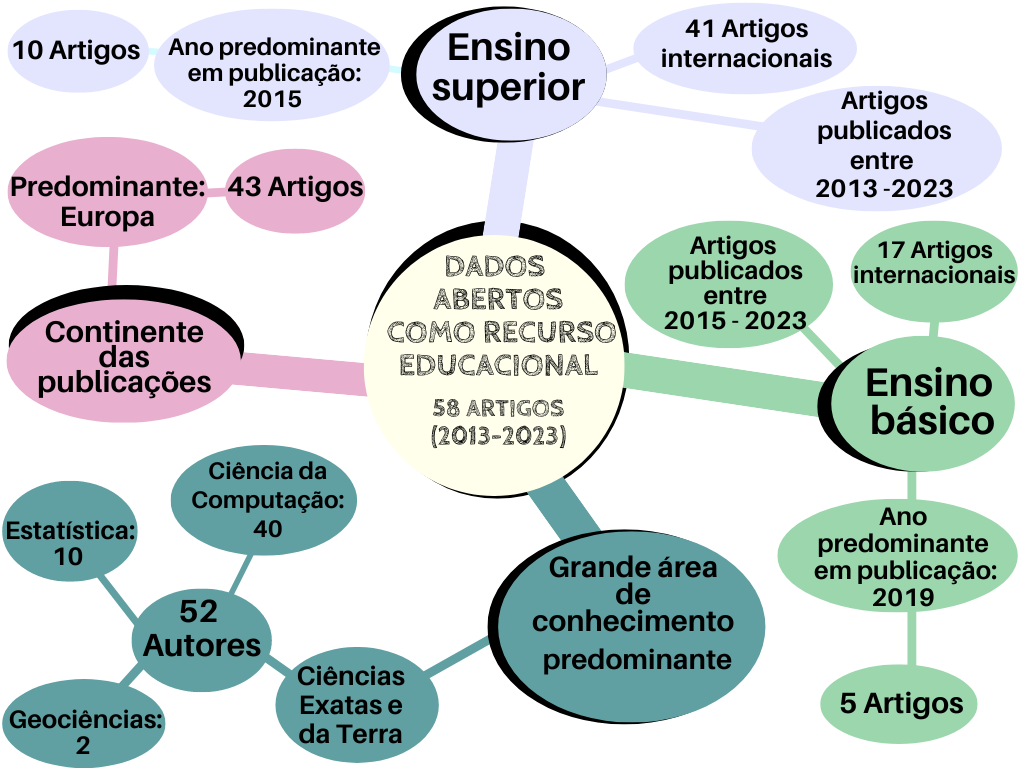
\includegraphics[width=\linewidth]{Fig7.png}
\caption{Síntese dos resultados predominantes.}
\label{fig7}
\source{Elaborado pela autora.}
\end{minipage}
\end{figure}

\section{Considerações finais}\label{sec-autores}
Esta pesquisa tem como objetivo responder à seguinte questão: quais são as tendências e características das publicações internacionais sobre o uso de dados abertos como instrumentos educacionais nos ensinos superior e básico, no período de 2013 a 2023?

Com base nos resultados apresentados, é possível delinear algumas constatações que respondem a essa questão, destacando tanto as dimensões quantitativas quanto qualitativas das publicações. Essas dimensões oferecem \textit{insights} significativos sobre as tendências e características dos artigos internacionais que investigam o emprego de dados abertos no contexto educacional durante o período analisado.

\textbf{Dimensão Quantitativa:}

\textbf{Produção Modesta}: O volume total de artigos, 41 no ensino superior e 17 no ensino básico, sinaliza uma modesta produção internacional.

\textbf{Áreas de Enfoque}: A grande área de Ciências Exatas e da Terra destacou-se no levantamento, com proeminência da subárea da Ciência da Computação, indicando um foco específico nessa disciplina na integração de dados abertos na educação.

\textbf{Geografia das Publicações}: A liderança da Europa com 43 artigos, revela uma tendência geográfica, sugerindo um maior interesse ou recursos investidos na interseção entre dados abertos e educação entre os pesquisadores europeus.

\textbf{Dimensão Qualitativa:}

\textbf{Potencialidades Abordadas}: os benefícios significativos reconhecidos na literatura apontam para a promoção de transparência, engajamento e inovação no contexto educacional. 

\textbf{Desafios Reconhecidos}: Desafios tais como privacidade e qualidade dos dados refletem a complexidade inerente à incorporação de dados abertos no cenário educacional e a necessidade de considerar cuidadosamente esses aspectos na implementação de iniciativas.

\textbf{Assimetria nas Produções Acadêmicas}: a assimetria ilustra possíveis disparidades regionais ou áreas de conhecimento mais propensas a explorar a temática, apontando para a necessidade de um olhar crítico sobre as condições que moldam essa assimetria.

\textbf{Limitações Temporais}: As conclusões baseiam-se na análise da produção acadêmica disponível até 2023. Recomenda-se considerar a dinâmica do campo, pois novas publicações e perspectivas podem ter surgido após esse período.

Em síntese, o levantamento contribui para a compreensão do estado atual das pesquisas internacionais sobre o tema. A produção modesta identificada evidencia a necessidade de ampliar e aprofundar as investigações nesse campo, com o objetivo de explorar o potencial transformador dos dados abertos na educação e superar os desafios inerentes à sua integração.

\section{Agradecimentos}\label{sec-idioma}
Agradeço ao Departamento de Letras e demais setores da UNICENTRO pela aprovação do Projeto de Pesquisa Isolado (PqI), que possibilitou este artigo, e aos professores Rodrigo Esteves de Lima-Lopes e Marcelo Buzato, do IEL, pelos ensinamentos e pelas novas possibilidades de investigação acadêmica proporcionadas.


\printbibliography\label{sec-bib}
%conceptualization,datacuration,formalanalysis,funding,investigation,methodology,projadm,resources,software,supervision,validation,visualization,writing,review

\end{document}
